\section{Thiết kế UI/UX}
\label{sec:ui-ux-design}

\begin{guide}
Phần này đặc tả thiết kế trải nghiệm và giao diện, đáp ứng chuẩn đầu ra L.O.2.1, L.O.2.2 và L.O.2.3 của môn học.
Mỗi quyết định thiết kế nên truy vết được về persona (mục~\ref{sec:user-personas}) và user story (mục~\ref{sec:user-stories}).
\end{guide}

\subsection{Kiến trúc thông tin và điều hướng}
\label{sec:information-architecture}

\begin{guide}
\guidepart{Nội dung}
\begin{compactitem}
    \item Sơ đồ điều hướng phân cấp (sitemap) của toàn ứng dụng: màn hình chính, 4 phân hệ và các màn hình con.
    \item Bottom Navigation Bar với tối đa 5 tab chính: những tab nào, thứ tự và biểu tượng.
    \item Navigation Drawer hoặc Modal Sheet cho các tác vụ phụ (tài khoản, cài đặt, \ldots), kết hợp thanh tìm kiếm và bộ lọc.
\end{compactitem}
\guidepart{Câu hỏi cần trả lời}
\begin{compactitem}
    \item Vì sao chọn các tab này cho Bottom Navigation Bar? Tab nào là màn hình mặc định khi mở ứng dụng?
    \item Từ màn hình chính, người dùng cần bao nhiêu lần chạm để tới nội dung dùng thường xuyên nhất?
    \item Tìm kiếm hoạt động riêng trong từng phân hệ hay tìm chung trên toàn bộ nội dung? Bộ lọc gồm những tiêu chí nào?
\end{compactitem}
\guidepart{Hình/bảng nên có}
Sơ đồ điều hướng (sitemap), wireframe của Bottom Navigation Bar và Navigation Drawer.
\end{guide}

\subsection{User Flows}
\label{sec:user-flows}

Phần này đặc tả các luồng thao tác chính bằng sơ đồ, so le giữa \textit{định nghĩa hành vi đã chốt} ở ma trận case C1--C9 (bảng~\ref{tab:switch-matrix}) và \textit{ảnh chụp thật từ ứng dụng}. Mỗi luồng được truy vết về user story ở mục~\ref{sec:user-stories} và về kịch bản kiểm thử TC01--TC14 của nhóm.

\textbf{Luồng phiên đầu tiên.} Đây là luồng quan trọng nhất vì quyết định người dùng có ``chạm'' được USP ngay lần đầu mở ứng dụng hay không. Hình~\ref{fig:act-first-run} mô tả luồng này bằng sơ đồ hoạt động theo đúng các con số đã chốt ở mục~\ref{sec:mvp-scope}.



Luồng phiên đầu tiên tuân theo ba nguyên tắc của onboarding: \textbf{giá trị}~--~ba màn đầu chỉ giải thích OneSpace giải quyết được gì (một app thay bốn app chuyên biệt) thay vì khoe tính năng; \textbf{quyền riêng tư}~--~không xin quyền nào lúc mở lần đầu, mọi quyền chỉ hỏi đúng lúc người dùng dùng đến tính năng cần nó; và \textbf{tính liền mạch}~--~chọn chủ đề xong vào thẳng Home với đề xuất theo đúng chủ đề vừa chọn, không bắt đăng nhập trước khi thấy được sản phẩm (chế độ dùng thử luôn có).

\textbf{Xung đột âm thanh (case C1).} Khi người dùng mở một bài nhạc trong lúc video đang phát, ứng dụng hỏi bằng popup hai lựa chọn (tắt tiếng video / dừng video) kèm ô tick ``Không hỏi lại''; lựa chọn áp dụng cho lần đó và lần xung đột sau vẫn hỏi~--~chỉ khi người dùng tích ``Không hỏi lại'' thì lựa chọn đang chọn được ghi nhớ, và đặt lại ``Luôn hỏi'' được trong Cài đặt. Hình~\ref{fig:act-conflict} là sơ đồ hoạt động theo đúng định nghĩa đã chốt; Hình~\ref{fig:app-c1} là popup thật trên ứng dụng.



\begin{figure}[H]
\centering
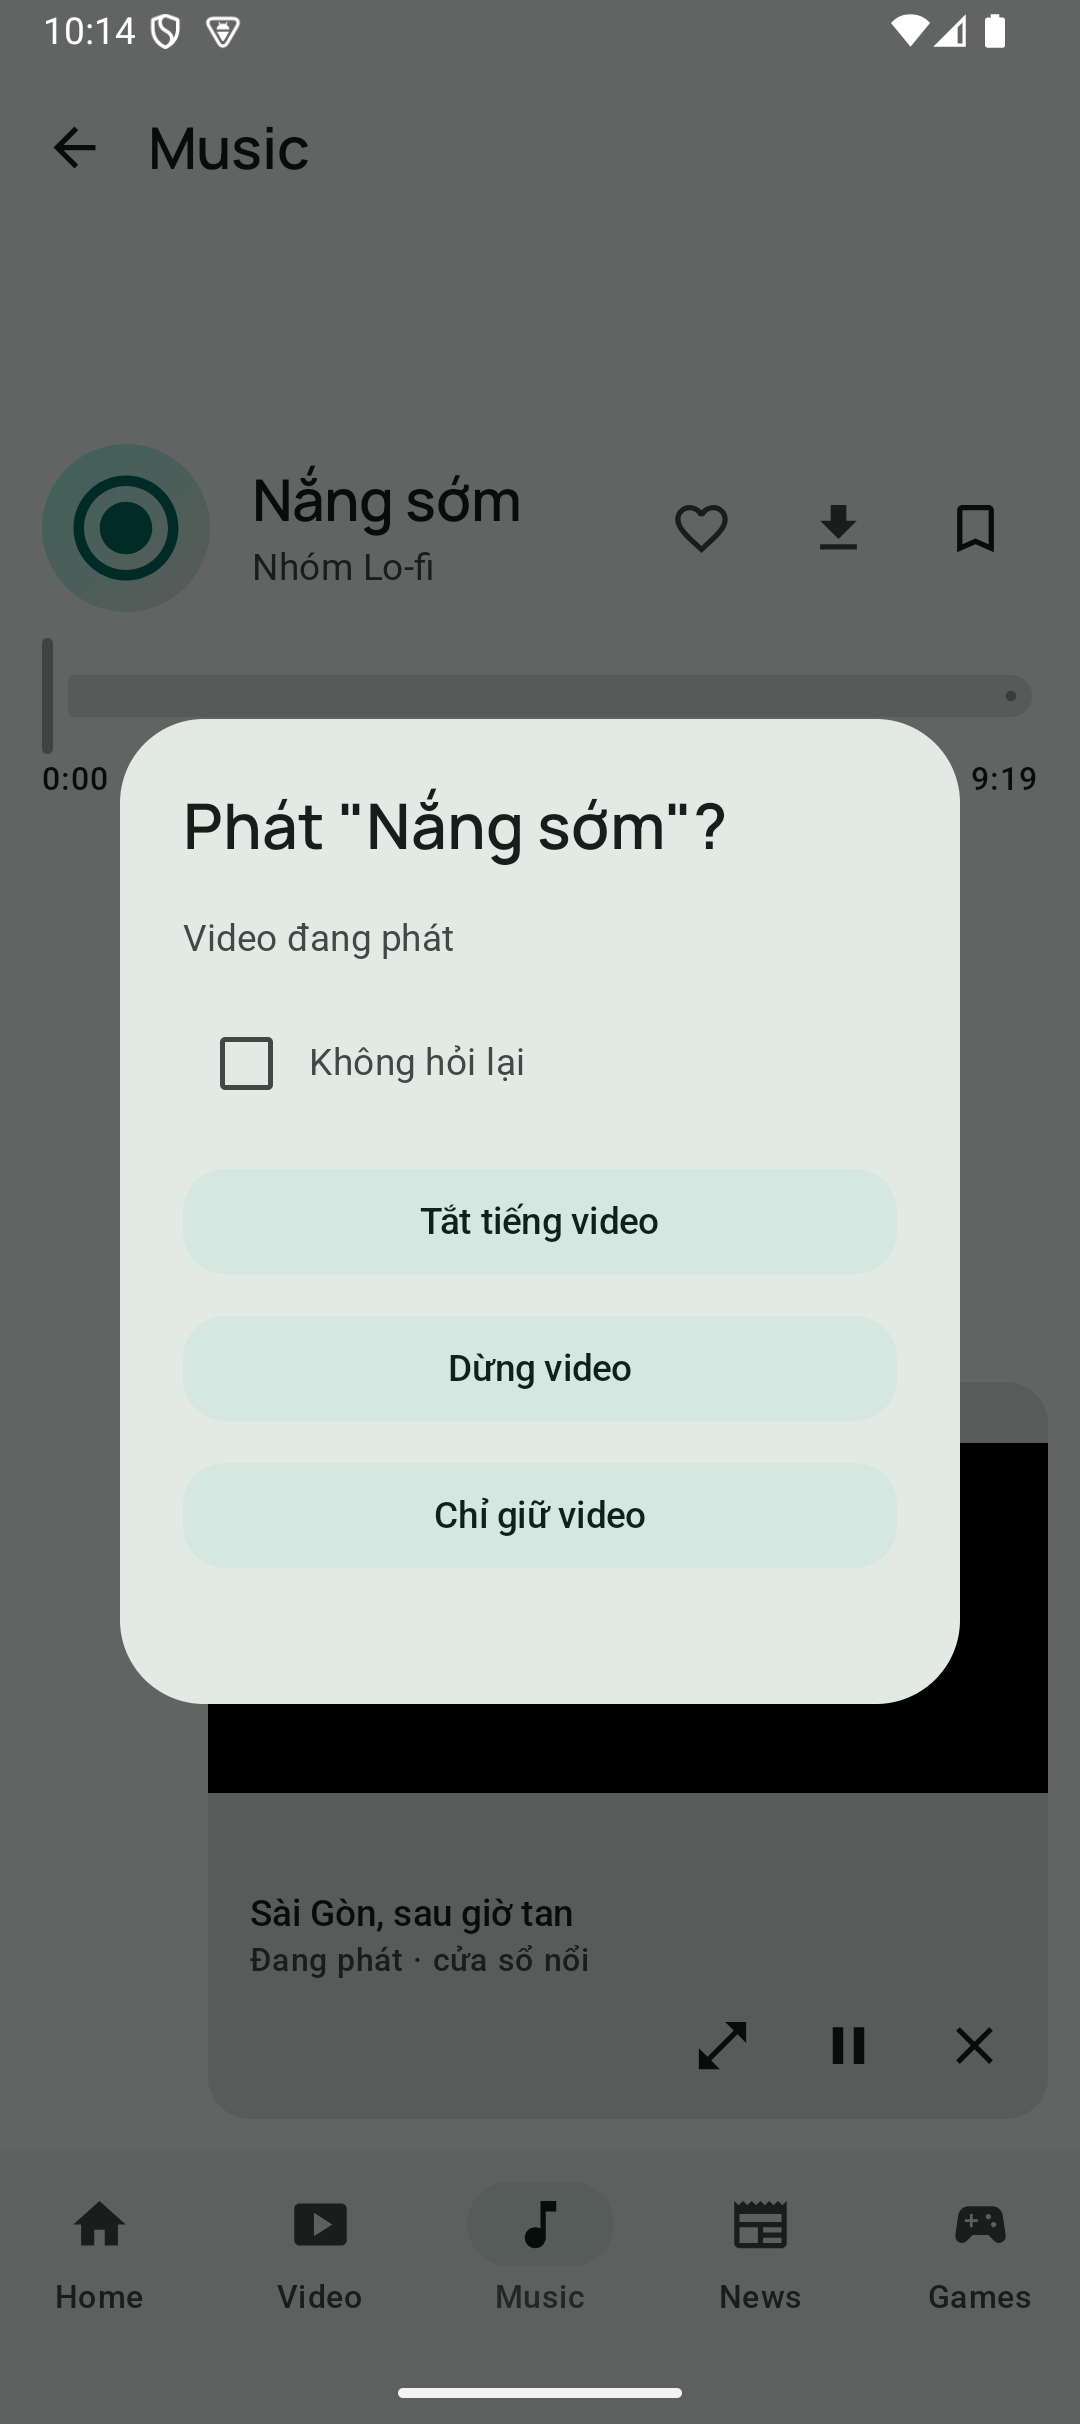
\includegraphics[width=0.28\textwidth]{figures/app/c1-audio-conflict-light.png}
\caption{Popup xung đột âm thanh thật trên ứng dụng: video ``Gần với thiên nhiên thêm chút'' đang phát, người dùng mở bài ``Nơi nào yên tĩnh''}
\label{fig:app-c1}
\end{figure}

Hình~\ref{fig:app-pip} chụp cửa sổ nổi thật đang chạy trên tab News: cửa sổ hiển thị tên video cùng các nút điều khiển, trong đó có Mở rộng, Tạm dừng và Đóng.

\begin{figure}[H]
\centering
\begin{minipage}{0.48\textwidth}
\centering
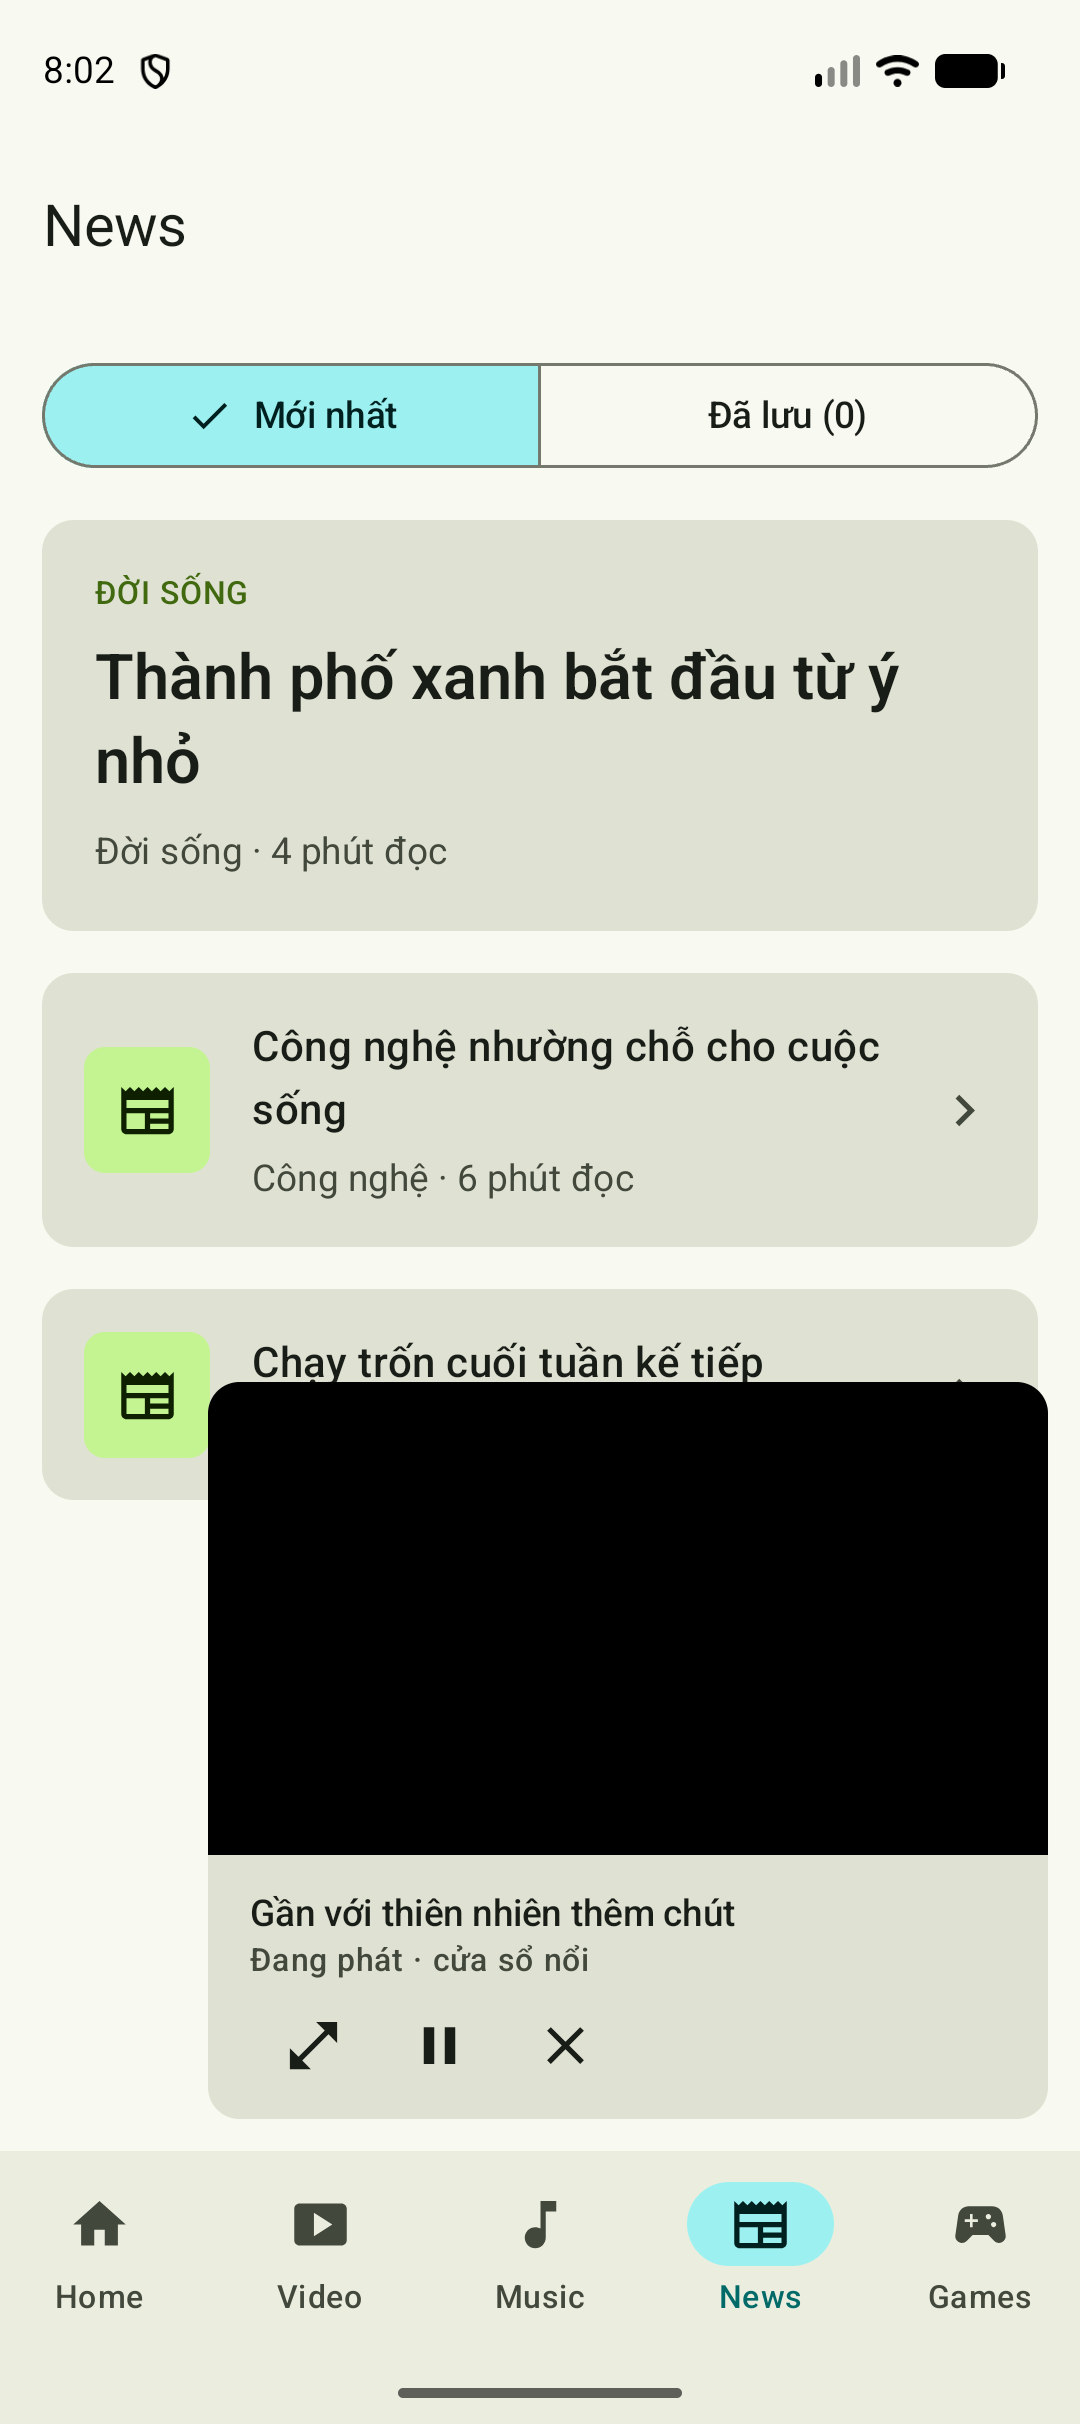
\includegraphics[width=0.55\textwidth]{figures/app/news-pip-light.png}
\caption{Video thu nhỏ thành cửa sổ nổi trên tab News (case C3, F-VID-08)}
\label{fig:app-pip}
\end{minipage}\hfill
\begin{minipage}{0.48\textwidth}
\centering

\includegraphics[width=0.55\textwidth]{figures/app/article-music-dock-light.png}
\caption{Dock mini player hiển thị trong trình đọc bài, nhạc vẫn phát khi đọc tin (case C7, F-NEWS-07)}
\label{fig:app-dock-reader}
\end{minipage}
\end{figure}

\textbf{Nghe nhạc khi đọc tin (case C7).} Đi tiếp chiều B$\rightarrow$C của C3, khi nhạc đang phát và người dùng sang tab News, dock mini player vẫn hiện trên feed và cả trong trình đọc bài để nhạc không bao giờ ``biến mất'' ngoài tầm điều khiển (Hình~\ref{fig:app-dock-reader}). Dock luôn hiển thị tên bài và nút tạm dừng; mở rộng dock ra trình phát đầy đủ cũng chỉ là một chạm.

\textbf{Khôi phục trạng thái.} Trong một phiên, SessionCoordinator giữ bài nhạc đang phát, video nổi và vị trí các màn hình khi người dùng chuyển tab. Khi tiến trình bị hệ điều hành hủy rồi mở lại, ứng dụng khôi phục tab cuối, bài nhạc cuối ở trạng thái dừng và danh sách phát; vị trí video trở lại khi người dùng mở lại đúng video đó nhờ checkpoint trong Room (Hình~\ref{fig:seq-restore}). Vị trí đọc tin, ván game dở qua process death và tự phát lại nhạc chưa được lưu, nằm trong danh sách kế hoạch; đây cũng là các dòng được đánh dấu trong bảng kiểm chứng kiến trúc.

Bảng~\ref{tab:flow-trace} tổng hợp việc truy vết từng luồng tới case, user story và bằng chứng tương ứng.

\begin{table}[H]
\centering
\caption{Truy vết luồng -- case -- user story}
\label{tab:flow-trace}
\begin{tabularx}{\textwidth}{>{\raggedright\arraybackslash}p{2.7cm} >{\raggedright\arraybackslash}p{1.4cm} >{\raggedright\arraybackslash}p{4.3cm} >{\raggedright\arraybackslash}X}
\toprule
\textbf{Luồng} & \textbf{Case} & \textbf{User story} & \textbf{Bằng chứng / kiểm thử} \\
\midrule
Phiên đầu tiên & -- & US-COM-02, US-COM-03 & Hình~\ref{fig:act-first-run} \\
Xung đột âm thanh & C1 & US-MUS-03, US-CROSS-02 & Hình~\ref{fig:act-conflict}, \ref{fig:app-c1}; TC02 \\
Video nổi khi rời tab & C3 & US-VID-02, US-CROSS-03 & Hình~\ref{fig:app-pip}; TC01 \\
Nghe nhạc khi đọc tin & C7 & US-NEWS-03, US-CROSS-01 & Hình~\ref{fig:app-dock-reader} \\
Nhạc tiếp tục khi vào game & C9 & US-GAME-01 & Dock vẫn hiện trên tab Games; TC04 \\
Khôi phục phiên (tab, bài cuối, vị trí video) & -- & US-CROSS-07 & Hình~\ref{fig:seq-restore}; TC05, TC10 \\
Mất mạng khi đọc tin / xem video & -- & US-CROSS-07 & mục~\ref{sec:wireframes-prototypes} \\
\bottomrule
\end{tabularx}
\end{table}

\textbf{Các nhánh lỗi và gián đoạn.} Nhánh ngoại lệ được định nghĩa bằng con số cụ thể để kiểm thử kết luận được ngay, thống nhất với bảng~\ref{tab:switch-matrix} và mục~\ref{sec:quality-pillars}: khi mất mạng giữa video, khung hình đứng kèm đếm ngược 5--15 giây tự thử lại; tin đã tải đọc tiếp; game offline chơi tiếp và điểm ghi cục bộ rồi đồng bộ khi có mạng. Khi mạng mất hẳn, feed chuyển sang trạng thái thông báo rõ ràng kèm nút ``Thử lại'' thay vì để màn hình trống trơn — trạng thái này được mô tả trong mục~\ref{sec:wireframes-prototypes}. Rút tai nghe: nhạc dừng ngay, không tự phát ra loa ngoài (TC12); cuộc gọi đến: mọi luồng nhường trong tối đa 0,5 giây và quay lại đúng chỗ sau cuộc gọi (TC11). Riêng nhánh ``nội dung chỉ dành cho tài khoản Premium'' không xuất hiện trong phiên bản đầu vì MVP phát hành miễn phí, không quảng cáo và không gói trả phí (quyết định ở mục~\ref{sec:mvp-scope}).

\subsection{Wireframe, Mockup và Prototype}
\label{sec:wireframes-prototypes}

\begin{guide}
\guidepart{Nội dung}
\begin{compactitem}
    \item Low-Fidelity (Lo-Fi): bản phác thảo nhanh bố cục các màn hình chính, chưa có màu sắc và hình ảnh thật.
    \item High-Fidelity (Hi-Fi): giao diện hoàn chỉnh với màu sắc, font chữ và hình ảnh theo design system ở mục~\ref{sec:design-system}.
    \item Interactive Prototype: bản mô phỏng có thể bấm được (clickable), kèm link để xem.
\end{compactitem}
\guidepart{Câu hỏi cần trả lời}
\begin{compactitem}
    \item Những màn hình nào được thiết kế, và chúng bao phủ các luồng nào ở mục~\ref{sec:user-flows}?
    \item Thiết kế đã thay đổi gì từ Lo-Fi sang Hi-Fi, và vì sao (dựa trên góp ý hay kết quả kiểm thử)?
    \item Prototype được dùng để kiểm thử với ai, và kết quả ra sao?
\end{compactitem}
\guidepart{Hình/bảng nên có}
Ảnh Lo-Fi và Hi-Fi đặt cạnh nhau cho từng màn hình chính, link tới prototype.
\end{guide}

\subsection{Design System}
\label{sec:design-system}

% Ô màu cho bảng token
\newcommand{\sw}[2]{\colorbox[HTML]{#1}{\textcolor[HTML]{#2}{\rule{0pt}{0.35cm}\hspace{0.7cm}}}}

Design system của OneSpace được xây trên \textbf{Material 3}~\cite{material3} và tổ chức hoàn toàn theo \textit{token theo vai trò} (role-based): mã nguồn không-hardcode màu, mọi màn hình đều tham chiếu các vai trò màu của Material Theme (\texttt{primary}, \texttt{onSurface}, \texttt{surfaceContainer}, \ldots) được định nghĩa tập trung trong một tệp theme duy nhất của ứng dụng. Cách đặt tên theo vai trò này bảo đảm khi thay đổi bảng màu, toàn bộ giao diện cập nhật đồng loạt mà không cần sửa từng màn hình~--~đây cũng là câu trả lời cho câu hỏi tái sử dụng token khi lập trình: một token được khai báo một lần, dùng ở mọi nơi.

Bảng màu theo định hướng thương hiệu \textit{mint--teal trên nền xanh mực}: màu chính light là xanh lá đậm (đậm hơn nền một bậc), ở dark chuyển thành mint sáng; màu phụ là teal. Mọi vai trò đều được khai báo thành cặp \texttt{role/onRole} (chữ trên nền tương ứng) để component tự giữ tương phản đọc được ở cả hai chế độ. Bảng~\ref{tab:design-tokens} liệt kê các token tiêu biểu; giá trị hex lấy trực tiếp từ mã nguồn theme của ứng dụng.

\begin{table}[H]
\centering
\small
\caption{Design token màu theo vai trò Material 3}
\label{tab:design-tokens}
\begin{tabularx}{\textwidth}{@{}>{\raggedright\arraybackslash}p{3.5cm} >{\centering\arraybackslash}p{1.3cm} >{\raggedright\arraybackslash}X@{}}
\toprule
\textbf{Vai trò (Light / Dark)} & \textbf{Màu} & \textbf{Dùng cho} \\
\midrule
primary / onPrimary \newline 41690F / B8F36E & \sw{41690F}{B8F36E} & Nút chính, tab đang chọn, liên kết \\
primaryContainer \newline C3F491 / 334E00 & \sw{C3F491}{334E00} & Vùng nhấn mạnh, nền icon thẻ \\
secondary / onSecondary \newline 006A68 / 9BD8D1 & \sw{006A68}{9BD8D1} & Nút phụ, chip chuyên mục \\
tertiary / onTertiary \newline 566516 / BDE886 & \sw{566516}{BDE886} & Điểm nhấn phụ (gamification) \\
error / onError \newline BA1A1A / FFB4AB & \sw{BA1A1A}{FFB4AB} & Thông báo lỗi, nút thử lại \\
background / onBackground \newline F8FAF2 / 10140E & \sw{F8FAF2}{10140E} & Nền màn hình và chữ chính \\
surface / onSurface \newline F8FAF2 / 10140E & \sw{F8FAF2}{10140E} & Bề mặt card, thanh công cụ \\
surfaceVariant \newline DEE3D0 / 43483D & \sw{DEE3D0}{43483D} & Chữ phụ, nền chip \\
surfaceContainer\allowbreak{}High \newline E5E8D6 / 272F25 & \sw{E5E8D6}{272F25} & Card nổi, dock mini player \\
outline \newline 75796D / 8E927F & \sw{75796D}{8E927F} & Viền phân tách, gợi ý ô nhập \\
\bottomrule
\end{tabularx}
\end{table}

Hai quyết định quan trọng về màu:

\begin{itemize}
    \item \textbf{Chế độ tối đi theo hệ thống, có ghi đè thủ công.} Ứng dụng đọc chế độ tối của hệ điều hành làm mặc định (tương ứng F-COM-13); trong Cài đặt người dùng chọn được Sáng, Tối hoặc Theo hệ thống~--~tùy chọn này được lưu và áp dụng cho toàn bộ ứng dụng ở lần mở sau.
    \item \textbf{Dynamic color tắt mặc định.} Android 12+ cho phép lấy màu theo hình nền của người dùng (dynamic color); ứng dụng hỗ trợ cơ chế này nhưng tắt mặc định để nhận diện thương hiệu mint--teal ổn định trên mọi thiết bị, vì bảng màu là một phần nhận diện sản phẩm chứ không phải trang trí.
\end{itemize}

Hình~\ref{fig:design-modes} so sánh cùng ba màn hình ở hai chế độ: cùng một hệ vai trò token giữ bố cục nguyên vẹn, chỉ đổi giá trị màu.

\begin{figure}[H]
\centering
\begin{minipage}{0.31\textwidth}\centering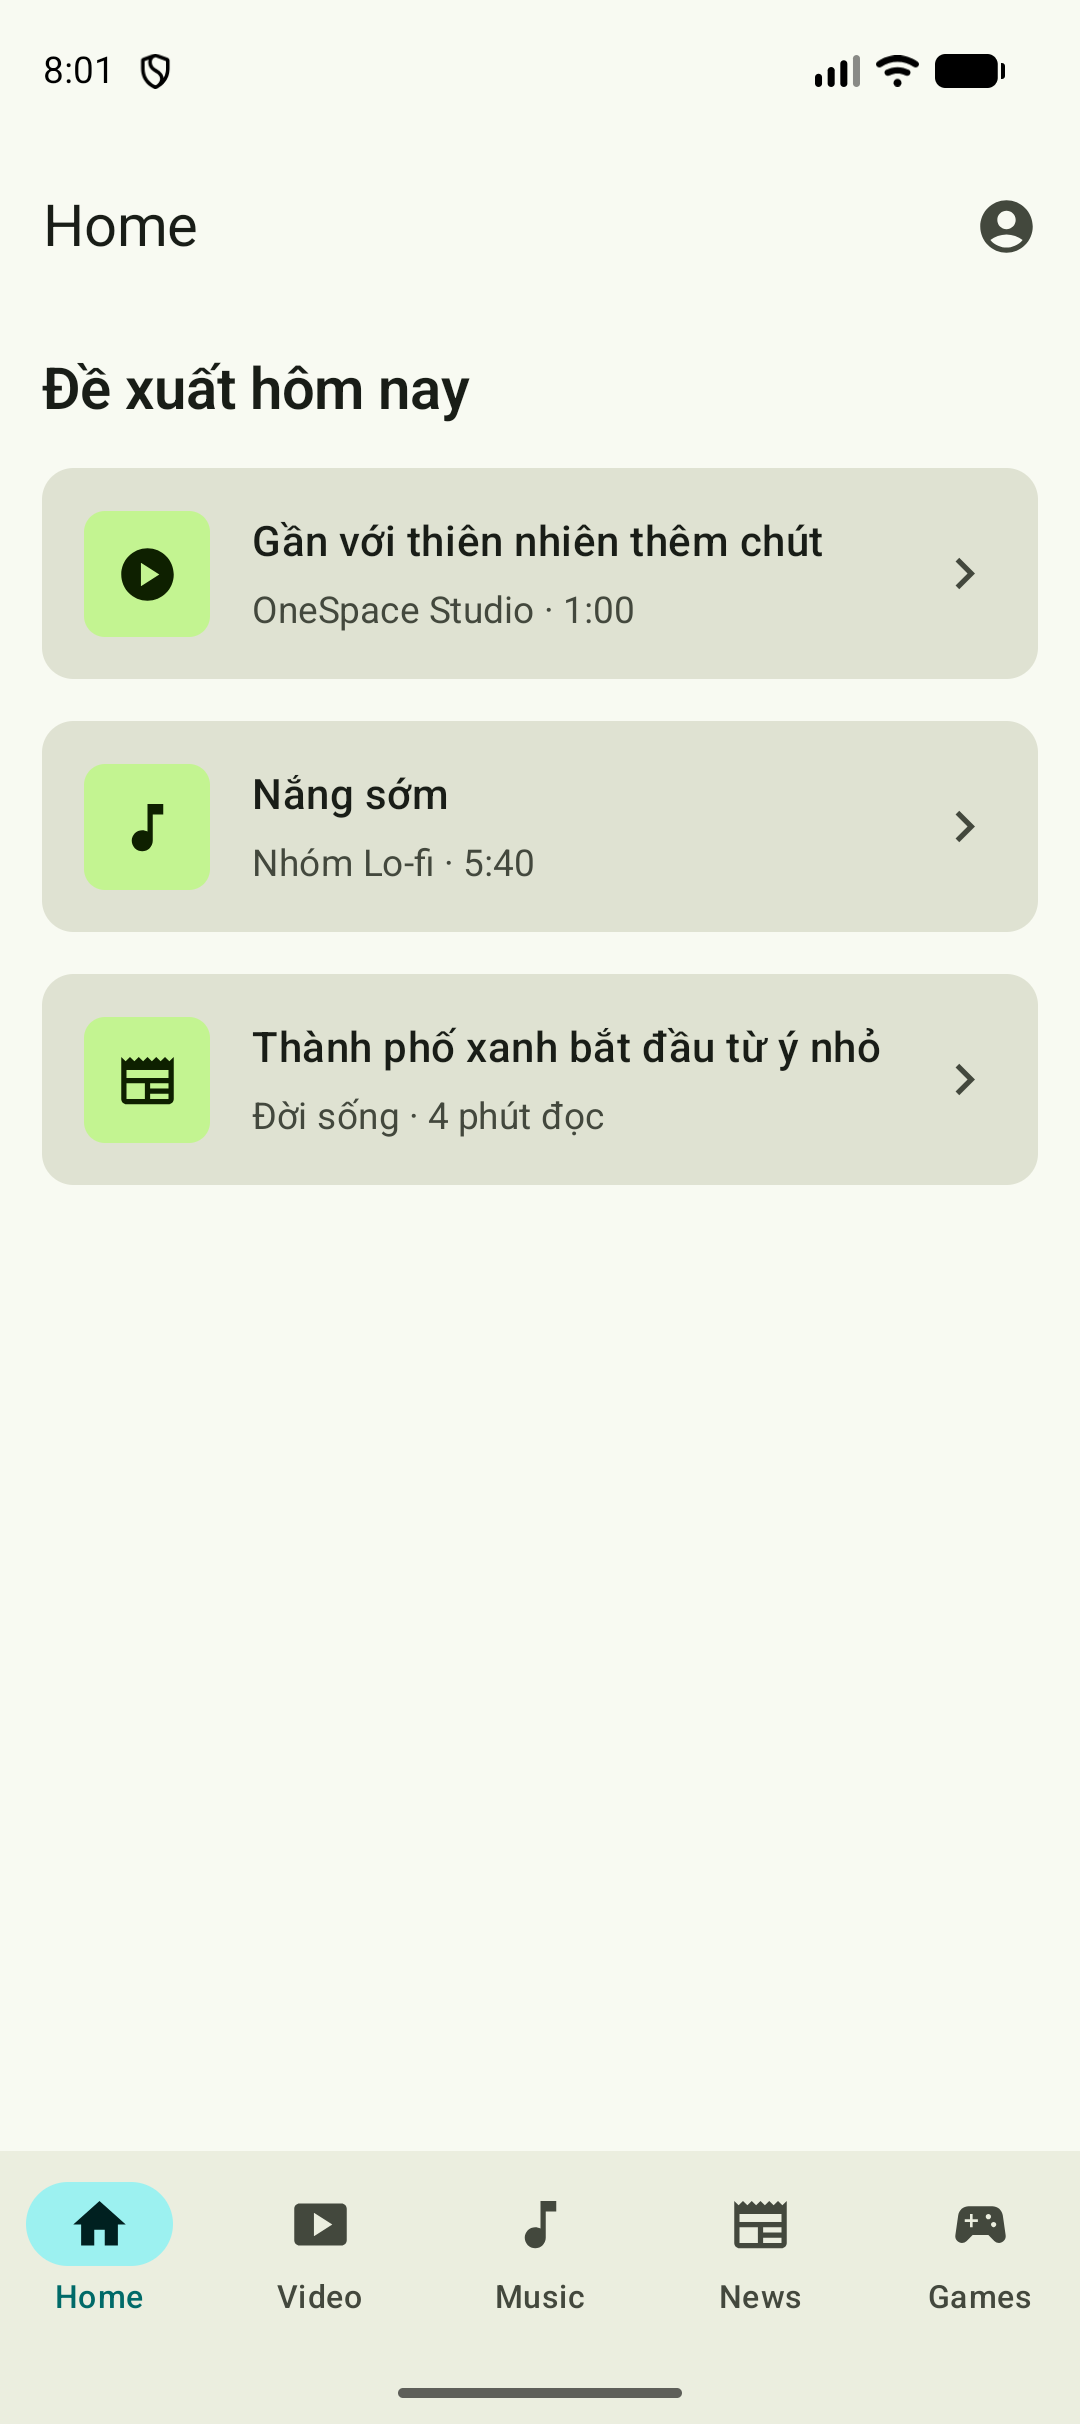
\includegraphics[width=0.86\textwidth]{figures/app/home-light.png}\end{minipage}\hfill
\begin{minipage}{0.31\textwidth}\centering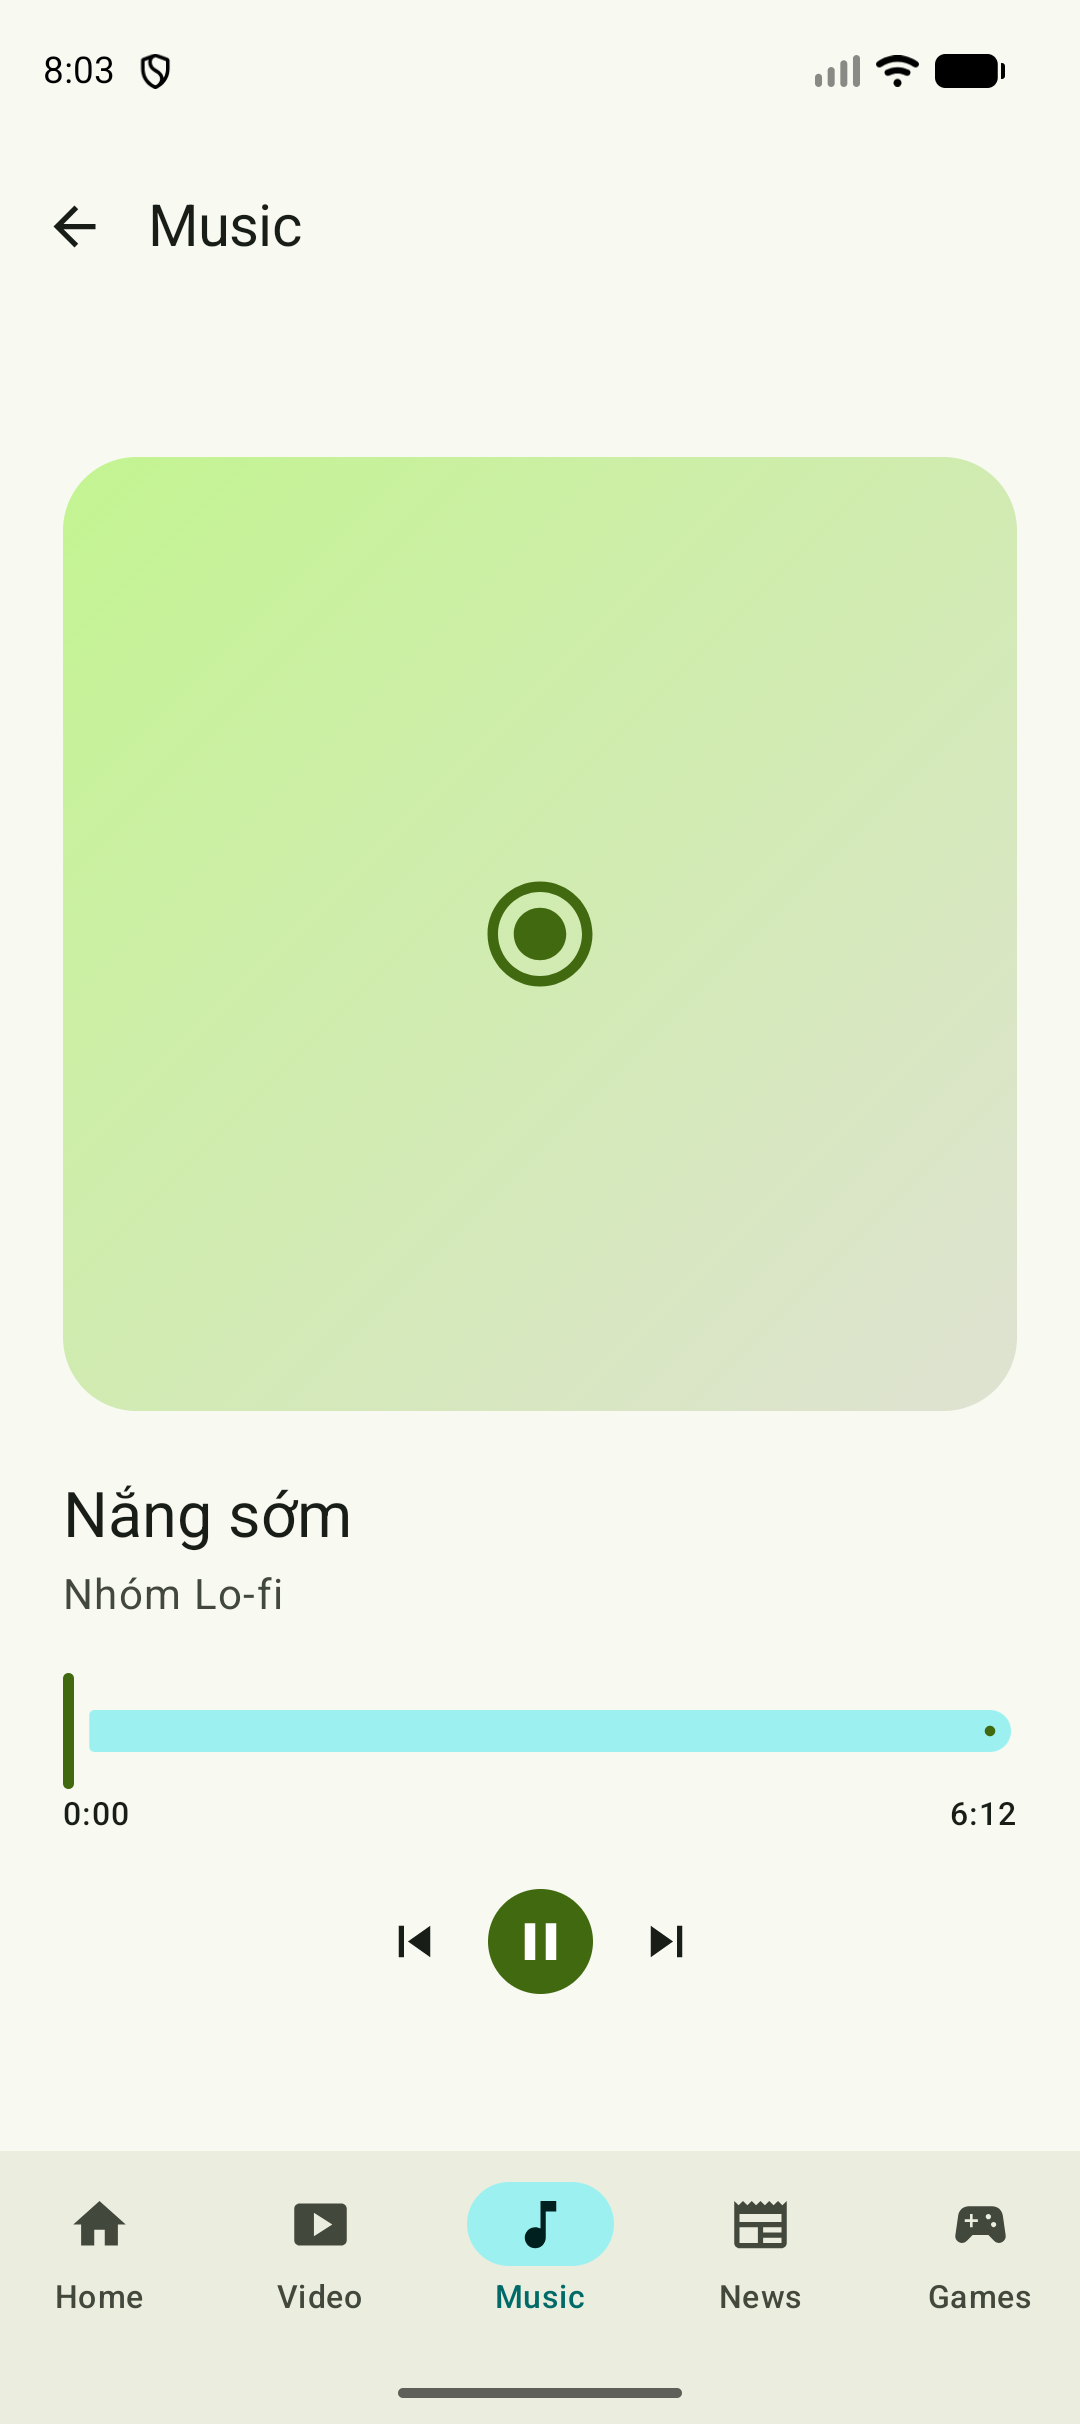
\includegraphics[width=0.86\textwidth]{figures/app/now-playing-light.png}\end{minipage}\hfill
\begin{minipage}{0.31\textwidth}\centering
\includegraphics[width=0.86\textwidth]{figures/app/article-light.png}\end{minipage}

\vspace{4pt}

\begin{minipage}{0.31\textwidth}\centering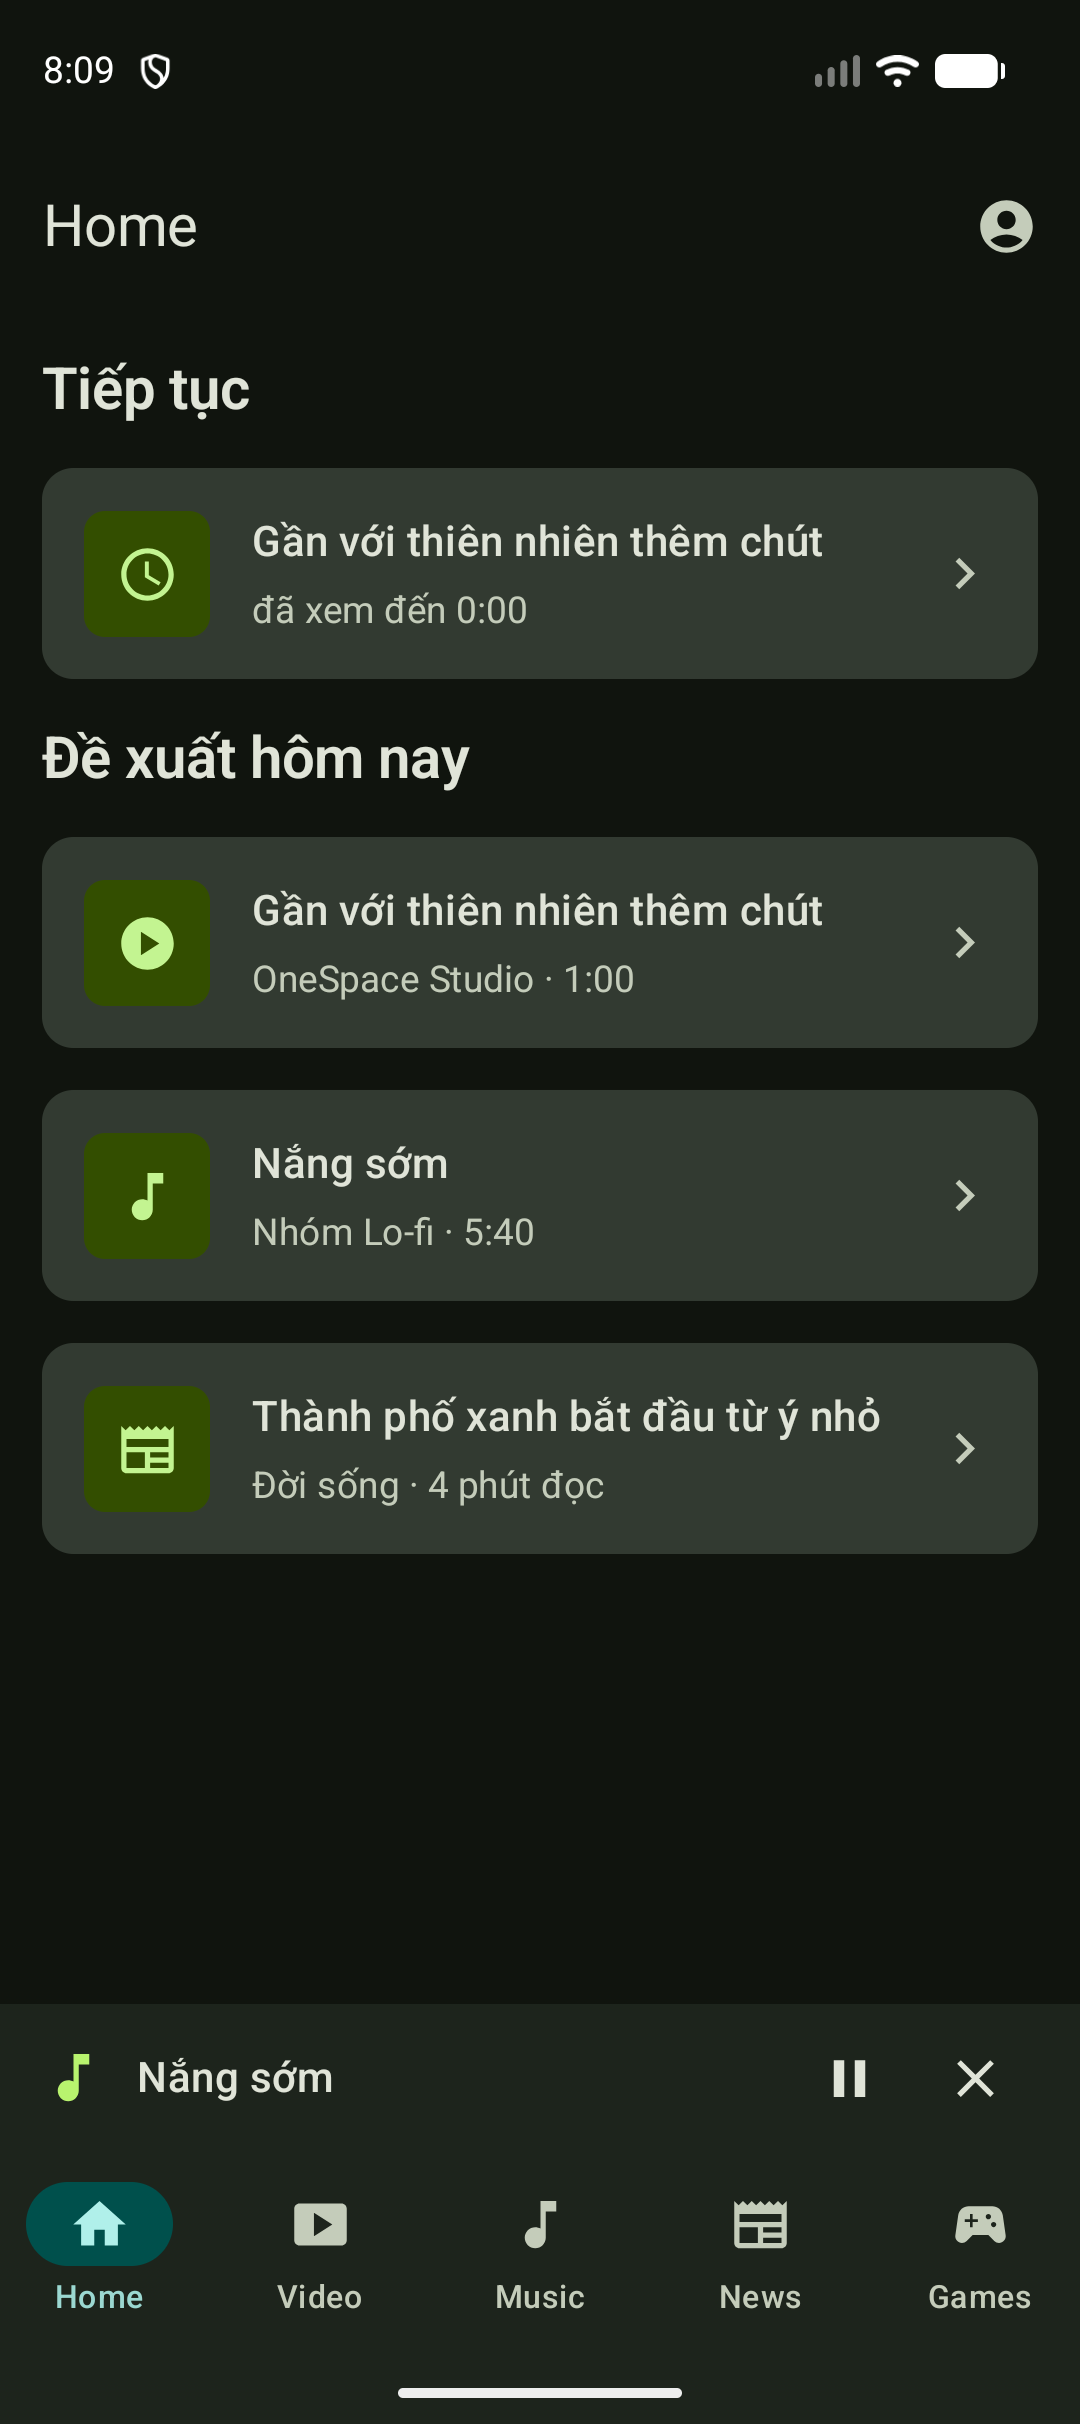
\includegraphics[width=0.86\textwidth]{figures/app/home-dark.png}\end{minipage}\hfill
\begin{minipage}{0.31\textwidth}\centering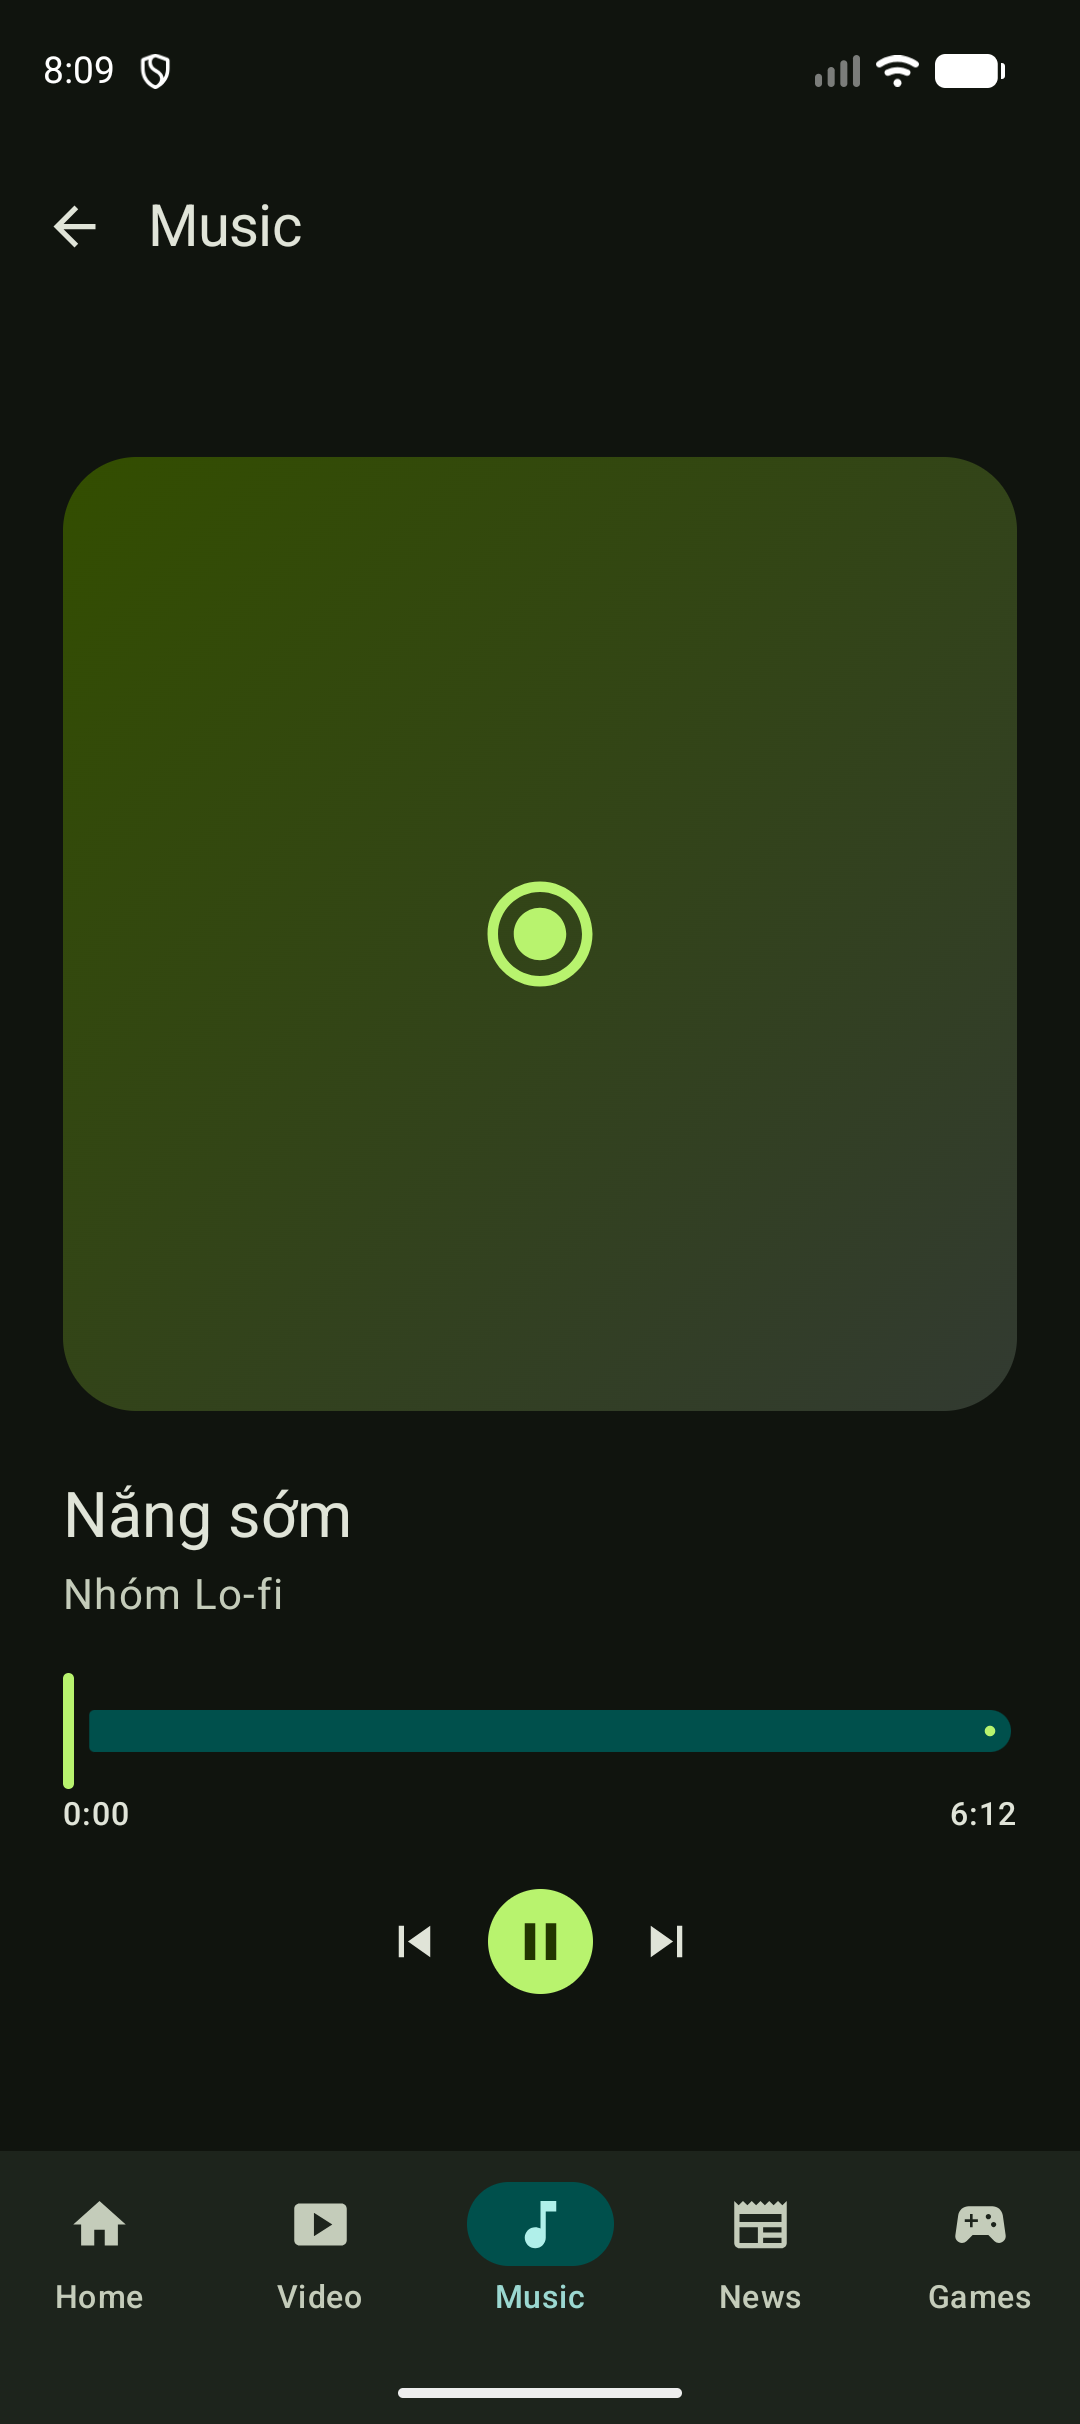
\includegraphics[width=0.86\textwidth]{figures/app/now-playing-dark.png}\end{minipage}\hfill
\begin{minipage}{0.31\textwidth}\centering
\includegraphics[width=0.86\textwidth]{figures/app/article-dark.png}\end{minipage}
\caption{Cùng ba màn hình ở chế độ sáng (trên) và tối (dưới): token giữ nguyên vai trò, chỉ đổi giá trị}
\label{fig:design-modes}
\end{figure}

\textbf{Typography.} Ứng dụng dùng nguyên thang chữ mặc định của Material 3 (display, headline, title, body, label) mà không định nghĩa kiểu chữ riêng. Quyết định này có chủ đích: thang M3 đã được hiệu chỉnh theo chuẩn đọc của Android, và mọi cỡ chữ đều đặt theo đơn vị \texttt{sp} nên tự phóng to theo cài đặt cỡ chữ hệ thống (chi tiết ở mục~\ref{sec:accessibility}). Việc thay font thương hiệu riêng, nếu có, sẽ là một thay đổi token tập trung duy nhất ở tệp theme.

\textbf{Component library.} Bảng~\ref{tab:component-library} phân loại component của ứng dụng: lớp \textit{dùng chung} định nghĩa trong module design system và được cả bốn phân hệ tham chiếu (đây là phần ``thư viện'' thật sự của design system); lớp \textit{theo chuẩn Material 3} dùng trực tiếp component nền tảng; các màn đặc thù tự dựng từ hai lớp này.

\begin{table}[H]
\centering
\caption{Thư viện component của OneSpace}
\label{tab:component-library}
\begin{tabularx}{\textwidth}{>{\raggedright\arraybackslash}p{3.4cm} >{\raggedright\arraybackslash}X}
\toprule
\textbf{Component} & \textbf{Vai trò} \\
\midrule
\multicolumn{2}{l}{\textit{Dùng chung (module design system)}} \\
\texttt{FeaturePage} & Khung trang cho mọi feed: padding ngang 16dp, khoảng cách dọc 16dp giữa các phần. \\
\texttt{SectionTitle} & Nhãn tiêu đề phần trong feed (``Tiếp tục'', ``Đề xuất hôm nay'', ``Liên quan''). \\
\texttt{ContentCard} & Thẻ nội dung dùng chung cho cả bốn phân hệ: biểu tượng trong vùng primaryContainer, tiêu đề, phụ đề và nút mở. \\
\texttt{CatalogContent} & Bộ chuyển trạng thái của mọi feed: đang tải $\rightarrow$ skeleton, lỗi/offline $\rightarrow$ thông điệp + thử lại, rỗng $\rightarrow$ thông điệp + nút hành động, có dữ liệu $\rightarrow$ nội dung. \\
\texttt{SkeletonFeed} & Bốn hàng khung xám chạy hiệu ứng shimmer thay cho feed đang tải. \\
\texttt{EmptyState} / \texttt{ErrorState} & Trạng thái rỗng (kèm nút hành động) và trạng thái lỗi (kèm ``Thử lại''). \\
\midrule
\multicolumn{2}{l}{\textit{Theo chuẩn Material 3}} \\
Bottom Navigation, ListItem, Switch, Button / OutlinedButton, Modal Bottom Sheet & Thanh 5 tab, hàng cài đặt, công tắc, nút, sheet xác nhận chế độ dùng thử. \\
\midrule
\multicolumn{2}{l}{\textit{Đặc thù từng phân hệ}} \\
Trình phát video + cửa sổ nổi, Now Playing, trình đọc bài, bàn chơi 2048 & Tự dựng theo bố cục riêng, vẫn dùng token và component chung ở trên. \\
\bottomrule
\end{tabularx}
\end{table}

Về quy chuẩn nền tảng: ứng dụng Android-native tuân theo Material Design~\cite{material3} cho toàn bộ ngôn ngữ tương tác~--~ripple khi chạm, elevation của card và bottom sheet, vùng chạm tối thiểu 48dp, motion theo chuẩn M3. Nhóm không áp dụng song song Apple Human Interface Guidelines vì sản phẩm chỉ phát hành trên Android (quyết định chọn nền tảng ở Phần~\ref{sec:technical-architecture}); giữ một quy chuẩn nền tảng duy nhất cũng giúp giao diện nhất quán hơn là pha trộn hai bộ quy chuẩn khác nhau.

\subsection{Accessibility}
\label{sec:accessibility}

\begin{guide}
\guidepart{Nội dung}
\begin{compactitem}
    \item Kích thước vùng chạm tối thiểu (Touch Target Size): $48 \times 48$~dp trên Android, $44 \times 44$~pt trên iOS.
    \item Độ tương phản màu theo chuẩn WCAG mức AA~\cite{wcag22}: tối thiểu 4.5:1 với văn bản thường.
    \item Hỗ trợ Dynamic Text Scaling (cỡ chữ theo cài đặt hệ thống) và trình đọc màn hình (TalkBack trên Android, VoiceOver trên iOS).
\end{compactitem}
\guidepart{Câu hỏi cần trả lời}
\begin{compactitem}
    \item Các cặp màu chữ và nền trong design system (mục~\ref{sec:design-system}) đạt tỉ lệ tương phản bao nhiêu? Kiểm tra bằng công cụ nào?
    \item Bố cục có bị vỡ khi người dùng đặt cỡ chữ hệ thống lớn nhất không?
    \item Các nút chỉ có biểu tượng đã có nhãn cho trình đọc màn hình (content description, accessibility label) chưa?
    \item Video có phụ đề không? Minigame có cách chơi thay thế cho người dùng trình đọc màn hình không?
\end{compactitem}
\guidepart{Hình/bảng nên có}
Bảng kiểm tra độ tương phản các cặp màu, checklist accessibility cho từng màn hình.
\end{guide}

\subsection{Micro-interactions và phản hồi tức thì}
\label{sec:micro-interactions}

Mỗi tương tác nhỏ của OneSpace được thiết kế theo mô hình bốn thành phần của Saffer~\cite{saffer2013}: \textit{Trigger} (điều kiện khởi động), \textit{Rules} (logic quyết định điều gì xảy ra), \textit{Feedback} (hiệu ứng người dùng nhìn thấy) và \textit{Loops \& Modes} (lặp lại và điều kiện đặc biệt). Bảng~\ref{tab:micro-interactions} liệt kê các micro-interaction đã cài đặt trong ứng dụng, chỉ gồm những tương tác có thật trong mã nguồn.

\begin{table}[H]
\centering
\small
\caption{Các micro-interaction của OneSpace theo mô hình bốn thành phần của Saffer}
\label{tab:micro-interactions}
\begin{tabularx}{\textwidth}{>{\raggedright\arraybackslash}p{2.6cm} >{\raggedright\arraybackslash}p{2.6cm} >{\raggedright\arraybackslash}p{3.2cm} >{\raggedright\arraybackslash}p{2.9cm} >{\raggedright\arraybackslash}X}
\toprule
\textbf{Tên} & \textbf{Trigger} & \textbf{Rules} & \textbf{Feedback} & \textbf{Loops \& Modes} \\
\midrule
Skeleton feed & Vào feed khi dữ liệu đang tải & Bốn hàng khung gồm một ô vuông và hai vạch ngang & Hiệu ứng shimmer (gradient chạy) trên khung xám & Dừng ngay khi có dữ liệu; chỉ dùng cho feed nhiều thông tin, không dùng cho thao tác nhẹ \\
\midrule
Ripple Material & Chạm mọi nút, thẻ, tab & Hiệu ứng chuẩn Material 3 & Vòng sóng lan từ điểm chạm & Mặc định toàn hệ thống \\
\midrule
Dock mini player & Bắt đầu phát một bài & Bài đang phát luôn hiện một hàng dock ở đáy nội dung & Dock hiện tên bài, nút tạm dừng và nút đóng & Dock hiện trên mọi feed và trong trình đọc bài; mở rộng thành trình phát đầy đủ bằng một chạm \\
\midrule
Thu nhỏ video thành cửa sổ nổi & Bấm ``Thu nhỏ \& khám phá'' hoặc rời tab khi video đang phát & Video tiếp tục phát trong cửa sổ nhỏ ở góc & Cửa sổ kèm nhãn ``Đang phát'' và ba nút: Mở rộng, Tạm dừng, Đóng & Quay lại trình phát đầy đủ giữ nguyên vị trí; đóng thì dừng hẳn \\
\midrule
Popup xung đột âm thanh & Mở nhạc khi video đang phát, lần đầu của cặp nội dung & Ba lựa chọn; lựa chọn được lưu theo cặp (case C1) & Hộp thoại liệt kê video đang phát kèm ba nút hành động & Từ lần thứ hai của cùng cặp: áp dụng im lặng, không hỏi lại \\
\midrule
Trạng thái rỗng & Mở danh mục không có nội dung (``Đã lưu'') & Hiển thị thông điệp kèm một hành động thoát khỏi tình huống & Biểu tượng, tiêu đề và nút ``Xem tin mới nhất'' & Không bao giờ để màn hình trống trơn không lối đi \\
\midrule
Trạng thái mất mạng & Feed không tải được dữ liệu & Hiển thị thông điệp ``Không có kết nối'' & Nút ``Thử lại'' ở giữa màn hình & Nhấn thử lại để tải lại; khi có mạng tự phục hồi \\
\midrule
Bàn chơi 2048 & Vuốt trên bàn chơi & Ô cùng giá trị gộp nhau theo hướng vuốt & Bàn chơi và điểm số cập nhật tức thì sau mỗi nước & Điểm cao nhất được ghi lại và hiện ở đầu màn chơi \\
\bottomrule
\end{tabularx}
\end{table}

\textbf{Quy tắc phản hồi và thời gian chờ.} Nguyên tắc xuyên suốt là \textit{giao diện không bao giờ đứng im khi chờ dữ liệu}: mọi thao tác đều có phản hồi tức thời trong ngưỡng 100~ms của \texttt{UX-01}~--~hiệu ứng ripple khi chạm, khung skeleton khi feed đang tải (mục~\ref{sec:wireframes-prototypes}). Việc phân biệt hai loại chỉ báo tuân theo quy tắc đặt ở mục~\ref{sec:quality-pillars}: \textit{skeleton} dùng cho màn hình nhiều thông tin (feed) vì người dùng thấy ngay hình dáng kết quả cuối sẽ ra sao; \textit{spinner/nút trạng thái} dùng cho thao tác nhẹ và ngắn (chuẩn bị quiz, đăng nhập). Khi thao tác thất bại, phản hồi chuyển từ ``đang chờ'' sang ``thông điệp lỗi + nút thử lại''. Gười dùng luôn có bước tiếp theo thay vì màn hình chết.

\textbf{Phản hồi xúc giác (haptic).} Ứng dụng hiện chưa sử dụng rung haptic: các tương tác đã đủ phản hồi thị giác rõ ràng ở giai đoạn này, và nhóm muốn tránh cảm giác rung gây khó chịu khi chưa có dữ liệu người dùng nào yêu cầu. Haptic được ghi nhận là hướng cân nhắc cho hai thời điểm có ý nghĩa rõ ràng nhất (ghép ô trong 2048 và trứng thú cưng nở), sẽ thêm sau khi có phản hồi từ người dùng thử nghiệm.

\textbf{Phản hồi âm thanh trong game.} Khi người dùng vào game trong lúc nhạc đang phát, hiệu ứng game không đè lên nhạc: theo quy tắc xử lý xung đột âm thanh ở mục~\ref{sec:mvp-scope}, nhạc được duck xuống (case C5)~--~phản hồi âm thanh vì vậy tuân theo cùng một bộ quy tắc với mọi luồng khác, thay vì mỗi phân hệ tự xử lý một kiểu.

%% [BỎ — heuristic evaluation là việc làm SAU khi có app thật, không phải lúc viết spec]
%% \label{sec:heuristic-evaluation}
%% 
%% \textbf{Phương pháp.} Ba thành viên của nhóm (Phạm Khánh Duy, Nguyễn Trần Yến Nhi, Tăng Hồng Ái) lần lượt duyệt độc lập giao diện của ứng dụng theo 10 nguyên lý usability của Nielsen~\cite{nielsen-heuristics}, mỗi người dùng cùng một bộ màn hình mockup ở mục~\ref{sec:wireframes-prototypes} và trực tiếp thao tác trên ứng dụng chạy emulator. Sau vòng duyệt độc lập, nhóm họp gộp các phát hiện trùng nhau, đánh giá mức độ nghiêm trọng theo thang 0--4 thường dùng kèm phương pháp này (0 = không phải vấn đề usability; 1 = vấn đề mỹ phẩm, chỉ nên sửa nếu còn thời gian; 2 = vấn đề nhỏ, ưu tiên thấp; 3 = vấn đề lớn, quan trọng để sửa, ưu tiên cao; 4 = thảm họa usability, bắt buộc phải sửa trước khi phát hành). Bảng~\ref{tab:heuristic-findings} liệt kê kết quả sau khi gộp.
%% 
%% \begin{table}[H]
%% \centering
%% \small
%% \caption{Kết quả heuristic evaluation: các phát hiện, mức độ và đề xuất}
%% \label{tab:heuristic-findings}
%% \begin{tabularx}{\textwidth}{>{\raggedright\arraybackslash}p{1.1cm} >{\raggedright\arraybackslash}p{2.9cm} >{\raggedright\arraybackslash}p{3.3cm} >{\centering\arraybackslash}p{0.9cm} >{\raggedright\arraybackslash}X}
%% \toprule
%% \textbf{Mã} & \textbf{Màn hình} & \textbf{Nguyên lý bị vi phạm} & \textbf{Mức} & \textbf{Đề xuất sửa} \\
%% \midrule
%% HE-01 & Home, Video, Onboarding, Games & 4. Consistency and standards & 3 & Thẻ game và một số nút chỉ có biểu tượng (Home, Onboarding, Video) chưa có nhãn \texttt{contentDescription}, và thẻ game không công khai trạng thái ``bấm được'' cho trình đọc màn hình~--~trong khi Account, Music, News đã có. Bổ sung nhãn cho mọi nút biểu tượng và ngữ nghĩa trạng thái bấm cho thẻ. \\
%% \midrule
%% HE-02 & Popup xung đột âm thanh (C1) & 6. Recognition rather than recall & 2 & Popup nêu tên video đang phát nhưng không nêu bài nhạc sắp được mở; người dùng phải nhớ mình vừa chọn bài nào. Thêm tên (và ảnh bìa) bài nhạc vào popup. \\
%% \midrule
%% HE-03 & Onboarding (ba bước) & 1. Visibility of system status & 2 & Không có chỉ báo tiến trình bước (1/3, 2/3, 3/3); người dùng không biết còn bao lâu thì xong. Thêm dải chấm hoặc nhãn bước. \\
%% \midrule
%% HE-04 & Cài đặt & 5. Error prevention & 2 & Công tắc ``Mô phỏng mất mạng (demo)'' là công cụ kiểm thử nhưng nằm ngay trong màn Cài đặt của người dùng; nếu bật nhầm, mọi feed sẽ lỗi mà không rõ nguyên nhân. Ẩn công tắc này trong bản phát hành chính thức. \\
%% \midrule
%% HE-05 & Toàn ứng dụng & 7. Flexibility and efficiency of use & 1 & Chưa có tìm kiếm; người dùng khám phá nội dung qua chuyên mục và đề xuất. Đã lên kế hoạch ô tìm xuyên nội dung (F-COM-11) ở giai đoạn sau MVP. \\
%% \midrule
%% HE-06 & Đăng nhập & 5. Error prevention & 1 & Ở bản demo, ô OTP chấp nhận mã bất kỳ nên không kiểm tra được luồng nhập sai. Khi nối xác thực thật, phải đặt giới hạn số lần sai và thời hạn mã đúng như \texttt{SEC-01}. \\
%% \bottomrule
%% \end{tabularx}
%% \end{table}
%% 
%% \textbf{Nhận xét.} Nguyên lý bị vi phạm nhiều nhất là \textit{Consistency and standards} (HE-01): một nửa số phân hệ đã gắn nhãn cho trình đọc màn hình còn một nửa chưa~--~chính sự thiếu nhất quán giữa các phân hệ, chứ không phải thiếu hẳn, làm vấn đề lộ rõ. Nguồn gốc là các phân hệ được làm song song bởi các thành viên khác nhau; bài học rút ra là các quy ước accessibility phải nằm trong component dùng chung của design system (mục~\ref{sec:design-system}) ngay từ đầu thay vì để từng màn hình tự quyết định.
%% 
%% Các phát hiện mức 1--2 đều đã có hướng xử lý cụ thể và không cản trở việc kiểm chứng USP. Phát hiện duy nhất mức 3 (HE-01) được xếp là \textbf{chưa sửa} ở phiên bản hiện tại: nhóm lập kế hoạch hoàn thành việc bổ sung nhãn cho toàn bộ nút biểu tượng và thẻ nội dung trong bản build kế tiếp, trước khi phát hành ra ngoài nhóm thử nghiệm. Không phát hiện nào đạt mức 4.
%% 
%% Bên cạnh các vấn đề, nhóm cũng ghi nhận các điểm giao diện vận hành tốt theo nguyên lý Nielsen, để giữ làm chuẩn khi tiếp tục phát triển: mọi trạng thái chờ đều có chỉ báo (nguyên lý 1~--~skeleton, dock luôn hiện bài đang phát); các hành động phá hủy đều có bước xác nhận (nguyên lý 3. Heet xác nhận chế độ dùng thử, popup C1); trạng thái rỗng và lỗi luôn kèm một hành động thoát khỏi tình huống thay vì dead-end (nguyên lý 9. Ỗ trợ khôi phục lỗi); và cùng một bộ component dùng chung trên bốn phân hệ khiến người dùng học cách dùng một lần thì dùng được ở mọi nơi (nguyên lý 4).
%% 
%% Giới hạn của đợt đánh giá này: người đánh giá là ba thành viên nhóm~--~cùng người thiết kế giao diện. Ên không loại trừ được thiên lệch quen biết; kết quả heuristic evaluation vì vậy được dùng để sàng lọc vấn đề rõ ràng trước, còn đánh giá với người dùng thật (năm người dùng, SUS) theo \texttt{UX-09} sẽ thực hiện ở giai đoạn kế tiếp như đã nêu ở mục~\ref{sec:heuristic-evaluation}.

